\documentclass[sigconf]{acmart}\settopmatter{printfolios=true,printccs=false,printacmref=false}
%\geometry{a4paper}

\usepackage[english]{babel}
\usepackage[utf8]{inputenc} % allow utf-8 input
\usepackage[T1]{fontenc}    % use 8-bit T1 fonts
%\usepackage[hidelinks]{hyperref}       % hyperlinks
\usepackage{url}            % simple URL typesetting
\usepackage{booktabs}       % professional-quality tables
\usepackage{amsfonts}       % blackboard math symbols
\usepackage{nicefrac}       % compact symbols for 1/2, etc.
\usepackage{microtype}      % microtypography
\usepackage{amsmath}
\usepackage{enumitem}
\usepackage{graphicx}
\usepackage{subcaption}
\usepackage{siunitx}
\usepackage{booktabs}
%\usepackage{float}
\usepackage{stfloats}
\usepackage{listings}
\colorlet{light-gray}{gray!20}

\sisetup{separate-uncertainty,detect-all}

\setcopyright{none}
\acmDOI{}
\acmISBN{}
\acmConference{Machine Learning for Healthcare}{2022}{ETH Zurich, Switzerland}
\copyrightyear{\today}


\begin{document}

\title{Project 2 Natural Language Processing}

\settopmatter{authorsperrow=3}
\author{Anton Schäfer}
\affiliation{
	\institution{ETH Zurich}
	\country{Switzerland}
}
\email{scanton@ethz.ch}

\author{Lasse F. Wolff Anthony}
\affiliation{
	\institution{ETH Zurich}
	\country{Switzerland}
}
\email{laanthony@ethz.ch}

\author{Nidhi Agrawal}
\affiliation{
	\institution{ETH Zurich}
	\country{Switzerland}
}
\email{agrawaln@ethz.ch}


\begin{abstract}
Cardiovascular diseases are the prime cause of human deaths. 
Analysis and processing of ECG signals are crucial for timely diagnosis of these diseases and other cardiac abnormalities. 
In this project work, we investigate automatic ECG interpretation using the PTB Diagnostic ECG Database and heart arrhythmia classification using the MIT-BIH Arrhythmia Database.
We develop several deep-learning based and traditional ML models and evaluate their performance across these tasks.
Finally, we show that transfer learning and ensemble methods can further improve performance but may inherit problems such as decreased performance across rare events or classes.
\end{abstract}


\maketitle

\section{Introduction}
A randomized controlled trial (RCT) is a study where participants from an eligible group are assigned randomly to an experimental group or a control group. The study tests the extent to which specific, planned impacts are being achieved. RCTs provide the most compelling medical evidence. Since there are massive amounts of RCT data available, automatic sequential sentence classification of this data will be very useful in literature reviews. NLP can also be used for automating other interesting use cases such as summarizing text, information extraction such as the scientific claim of an abstract or information retrieval such as effect of a drug on a disease.\\
In this work, we exploit NLP with traditional machine learning and deep learning and its capabilities to recognize complex data patterns, extract features automatically, and capture long range dependencies for PubMed 200k RCT dataset. We propose various machine learning, deep learning and transformer based models and evaluate their performance on this task and compare them. 
\label{sec:introduction}


\section{Models and Methods}
\label{sec:models_and_methods}
\subsection{Dataset}
We evaluate our models on an MRI imaging dataset and a dataset consisting of radiomics features extracted from these images:

\begin{itemize}[leftmargin=0cm]
    \setlength\itemsep{0.6em}
    \item[]
    \textbf{MRI images dataset:} The dataset consists images of 278 brain slices, 111 with tumor and 167 without any tumor, taken from the Kaggle datasets: Brain MRI Images for Brain Tumor Detection\footnote{\url{https://www.kaggle.com/datasets/navoneel/brain-mri-images-for-brain-tumor-detection}} and Brain Tumor Classification (MRI)\footnote{\url{https://www.kaggle.com/datasets/sartajbhuvaji/brain-tumor-classification-mri}}. Expert knowledge is not required to see the tumors in the images as they are clearly visible. The dataset is split into $250$ ($\sim$89\%) train and $28$ ($\sim$ 11\%) test samples. The images are labeled according to existence of tumor: 0 for no tumor and 1 for tumor.
    
    \item[]
    \textbf{Radiomics dataset:} This dataset has been automatically generated by extraction of radiomics features such as first-order statistics, texture, and shape from the aforementioned MRI images dataset using an open-source python package called pyradiomics\footnote{\url{https://pyradiomics.readthedocs.io/en/latest/}}. The split and class labels are identical.
    \end{itemize}

\subsection{Models}
We evaluate several interpretable models and post-hoc explanation methods with varying complexity to investigate the trade-off between model complexity, performance, and interpretability and explainability. In the following we outline the models and methods that we use:

\begin{itemize}[leftmargin=0cm]
    \setlength\itemsep{0.6em}
    \item[]
    \textbf{Random Forest:}
    We employ a simple random forest classifier \citep{breiman2001random} using the radiomics features as a baseline that prioritizes performance over interpretability (\textsc{Random Forest}). We add a permutation based post-hoc explanation method \citep{breiman2001random} to aid in visualizing which features were the most important during classification.\footnote{See \url{https://scikit-learn.org/stable/auto_examples/ensemble/plot_forest_importances.html}.}.\
    

    \item[]
    \textbf{Decision Tree:}
    A decision tree is arguable one of the most interpretable traditional ML models. The model and its training algorithm are easily understood, and we are able to interpret the model by visualizing the splits in each node. We introduce a decision tree model also trained on the radiomics features (\textsc{Decision Tree}) in contrast to the more complex \textsc{Random Forest} classifier and to highlight any potential performance cost of having a more interpretable tree-based model.
    
    \item[]
    \textbf{Logistic Regression:}
    Additionally, we train a simple logistic regression model (\textsc{Logistic Regression}) that lends itself to interpretation. We obtain a clear view of the important features used the model through its linear coefficients and their magnitude. This also allows us to see which features strongly predict or contribute to the tumor or no tumor prediction by their sign and magnitude. To further aid interpretability, we use L1 regularization to force coefficients of unhelpful features to 0.
    
    \item[]
    \textbf{Baseline CNN:}
    We train the provided baseline CNN model for increased accuracy over the simpler models (\textsc{Baseline CNN}). The trade-off we highlight here is model complexity, often leading to better performance, and interpretability. We add two post-hoc explanation methods, SHAP and LIME as described in the following section, to give a better understanding of the model and its predictions.
    
    
    \item[]
    \textbf{VGG16 TL:}
    Finally, we evaluate a VGG16 model with transfer learning (\textsc{VGG16 TL}). The model is pre-trained on the ImageNet dataset. We add three dense layers followed by a dropout layer and finally the output layer. All layers in the original model are frozen and then we fine-tune our added layers on the MRI image dataset. We further employ data augmentation to add some modifications to some of our input images by making minor changes, such as flipping, enhancing their contrast and sharpness leading to increased performance.
\end{itemize}
    
\subsection{Post-hoc Explanation Methods}
\begin{itemize}[leftmargin=0cm]
    \setlength\itemsep{0.6em}
    \item[]
    \textbf{SHAP:}    
    SHapley Additive exPlanations (SHAP) \citep{lundberg2017unified} is a model-agnostic approach that breaks down a prediction to show the impact of each feature. Image classification tasks are explained by attributing scores to each pixel on a predicted image. These scores indicate how much the pixels contribute to the probability of the image being classified in that particular class. Red pixels represent positive SHAP values that contributed positively to the classification of image as a particular class and blue pixels represent negative SHAP values which contributed to not classifying the image as that class.
    
    \item[]
    \textbf{LIME:}
    Local interpretable model-agnostic explanations (LIME) \citep{lime} is, like SHAP, a model-agnostic approach for explainability. LIME explains individual predictions of a classifier by learning an interpretable and faithful model locally around each prediction. In our task of brain tumor detection from MRI images, LIME produces images that explain our classifiers' predictions by highlighting the important region inside the image.
\end{itemize}



\section{Experiments}
\label{sec:experiments}

\begin{figure*}[t]
    \centering
    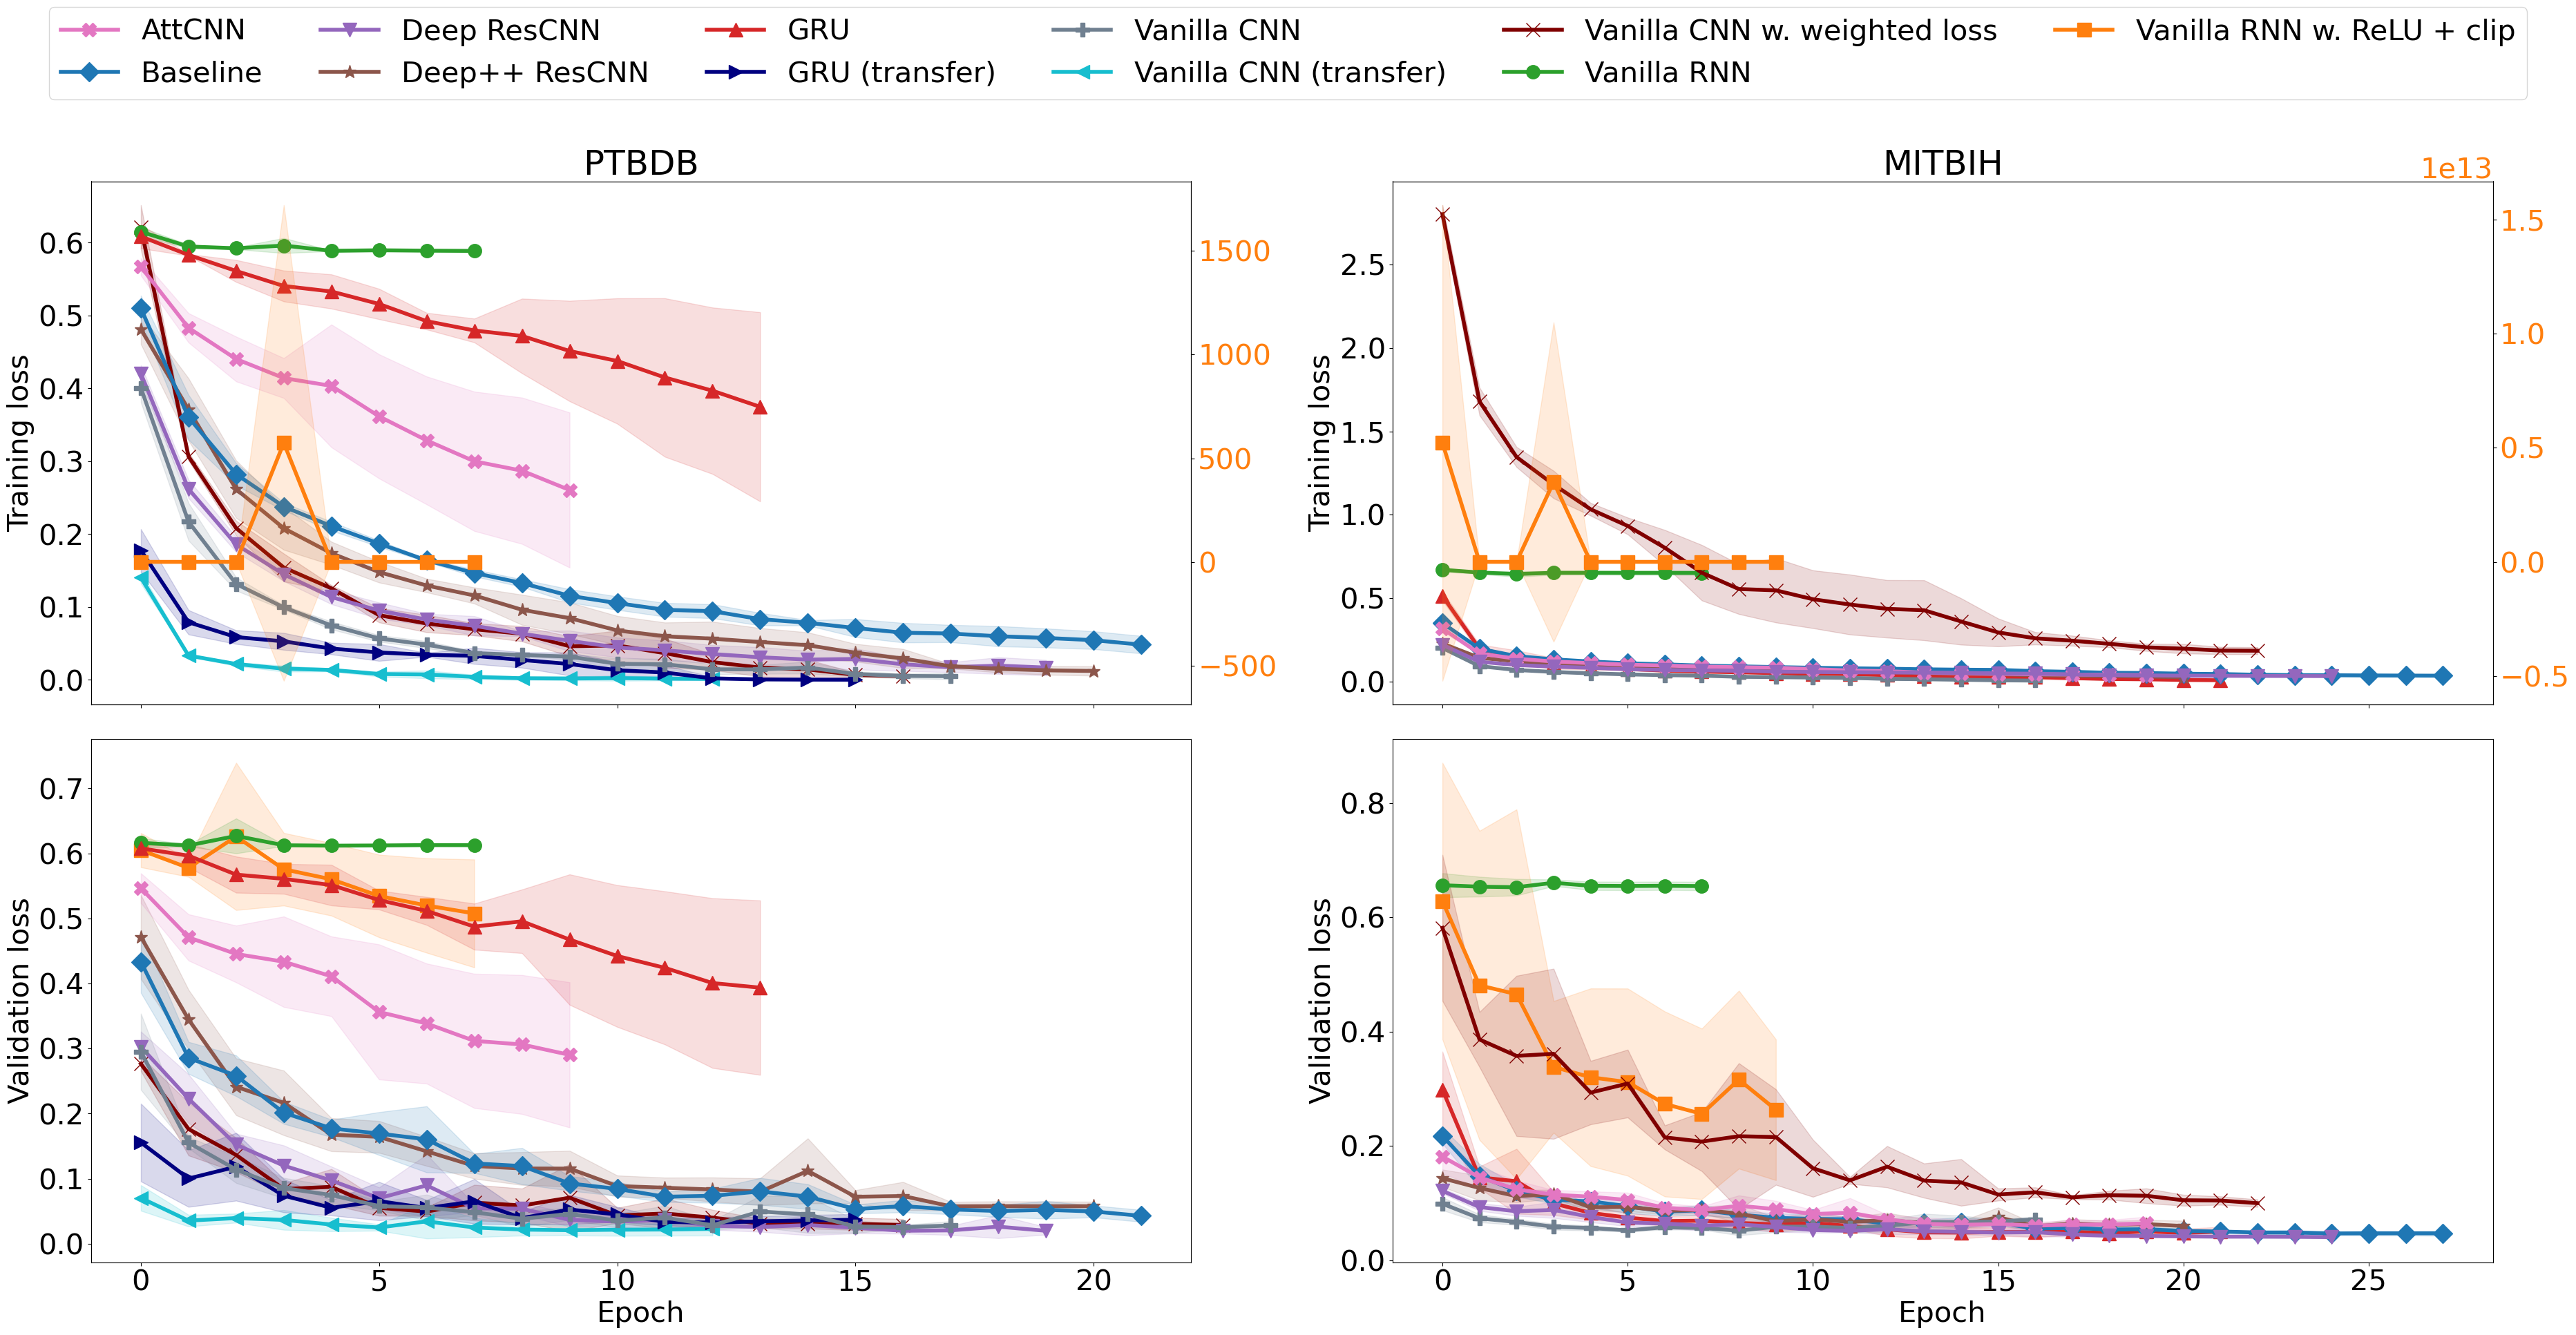
\includegraphics[width=0.70\textwidth]{figures/learning_curves.png}
    \caption{Learning curves for our deep-learning models showing the mean (upper) training and (lower) validation cross-entropy loss by epoch on the (left) PTB DB and (right) MIT-BIH datasets. The shaded areas depict \boldmath$\pm 1$ standard deviation from the mean. The second \boldmath$y$-axes (rhs) depicts the training loss for the Vanilla RNN w. ReLU + clip model.}
    \label{fig:learning_curves}
\end{figure*}

\subsection{Experimental Setup}
All of our experiments were performed on the ETH Euler cluster\footnote{\url{https://scicomp.ethz.ch/wiki/Euler}} using 1 unknown GPU and 1 unknown CPU with 8 GB of reserved RAM. We repeated every model run five times with consecutive seeds (seed 42 to 46) and report the mean and standard deviation. The tree-based models were developed using Scikit-learn \citep{scikit-learn}. The deep-learning models were developed using Tensorflow \citep{tensorflow2015-whitepaper} and were trained for a maximum of 1000 epochs using the Adam optimizer \citep{kingma2014adam} and decreasing the learning rate once validation accuracy plateaued for 3 epochs. We further used early stopping and assumed convergence when the validation accuracy showed no improvement for 7 (5 for baselines) consecutive epochs. The final models are the models with the highest validation accuracy.

Hyperparameter tuning was done using a random search \citep{bergstra2012random} over a large parameter space for both model and optimizer configurations. Optimal configurations can be found in the source code. We further experimented with Bayesian optimization to tune some models but this showed no improvement over a vast random search. It had a slightly higher compute efficiency but increased implementation complexity significantly.

For the MIT-BIH dataset, the F1-score is computed as the macro-averaged or unweighted mean of all per-class F1-scores. For the PTB DB dataset, we use AUPRC to denote the average precision score since directly computing the area under the precision-recall curve using the trapezoidal rule is prone to overestimating\footnote{See \url{https://scikit-learn.org/stable/modules/generated/sklearn.metrics.average_precision_score.html}.}



\subsection{Results and Discussion}

\subsubsection{Training behavior}
The training behavior of all deep-learning models models is shown in \autoref{fig:learning_curves}. As expected, larger models train slightly slower. They also exhibit greater variance in loss and final accuracy depending on the seeding. For the \textsc{VanillaRNN} model with Tanh activation and no gradient clipping, we find that it suffers from the vanishing gradient problem causing stagnating loss. \textsc{VanillaRNN+ReLU+Clip} performs much better, however, we observe divergence of loss, presumably due to large gradients, temporarily for some runs.

\begin{figure*}[t]
    \centering
    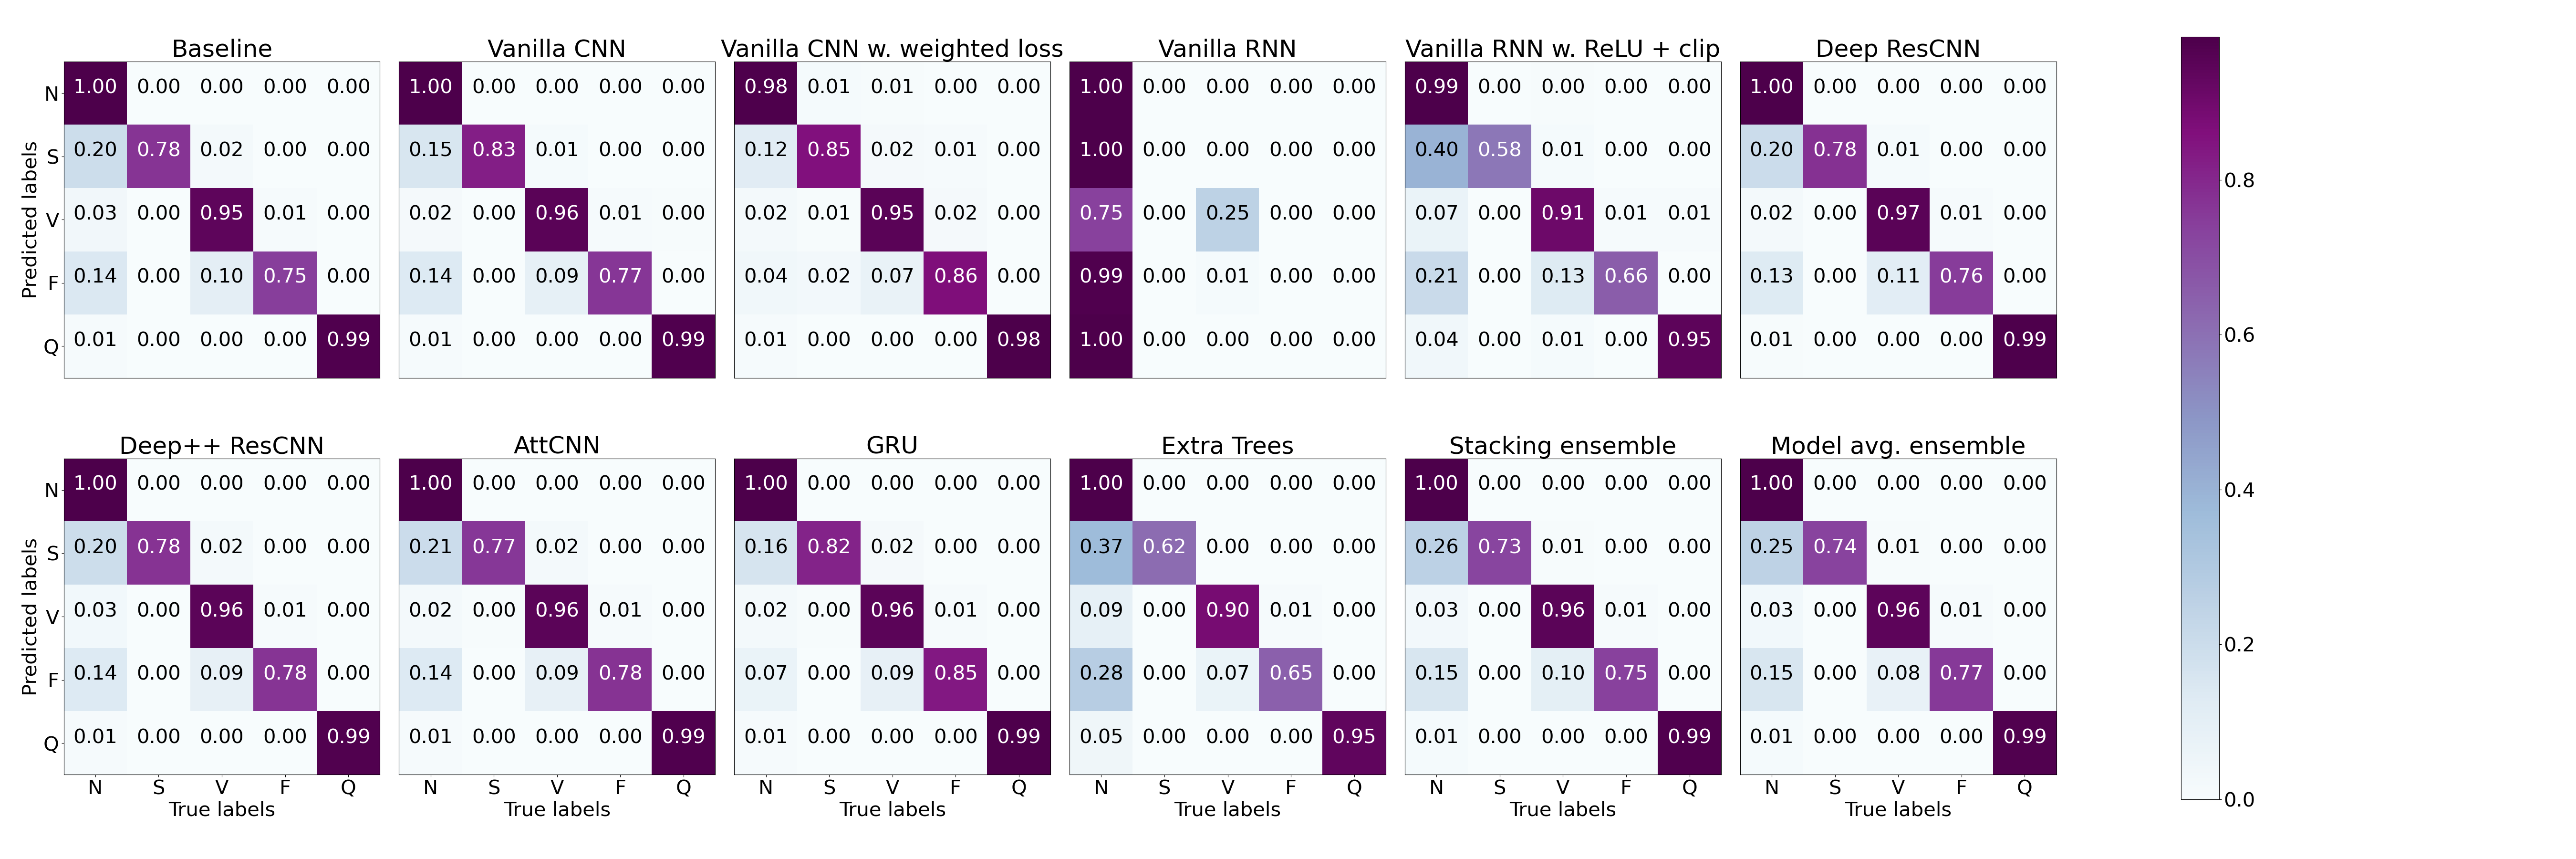
\includegraphics[width=1\textwidth]{figures/confusion_matrices_mitbih.png}
    \caption{Confusion matrices associated with our model performances on the MIT-BIH test dataset. The class abbreviations are as follows: 'N' is normal beat, 'S' is supraventricular premature beat, 'V' is premature ventricular contraction, 'F' is fusion of ventricular and normal beat, and 'Q' is unclassifiable beat.}
    \label{fig:confusion_matrices_mitbih}
\end{figure*}

\begin{figure}[]
    \centering
    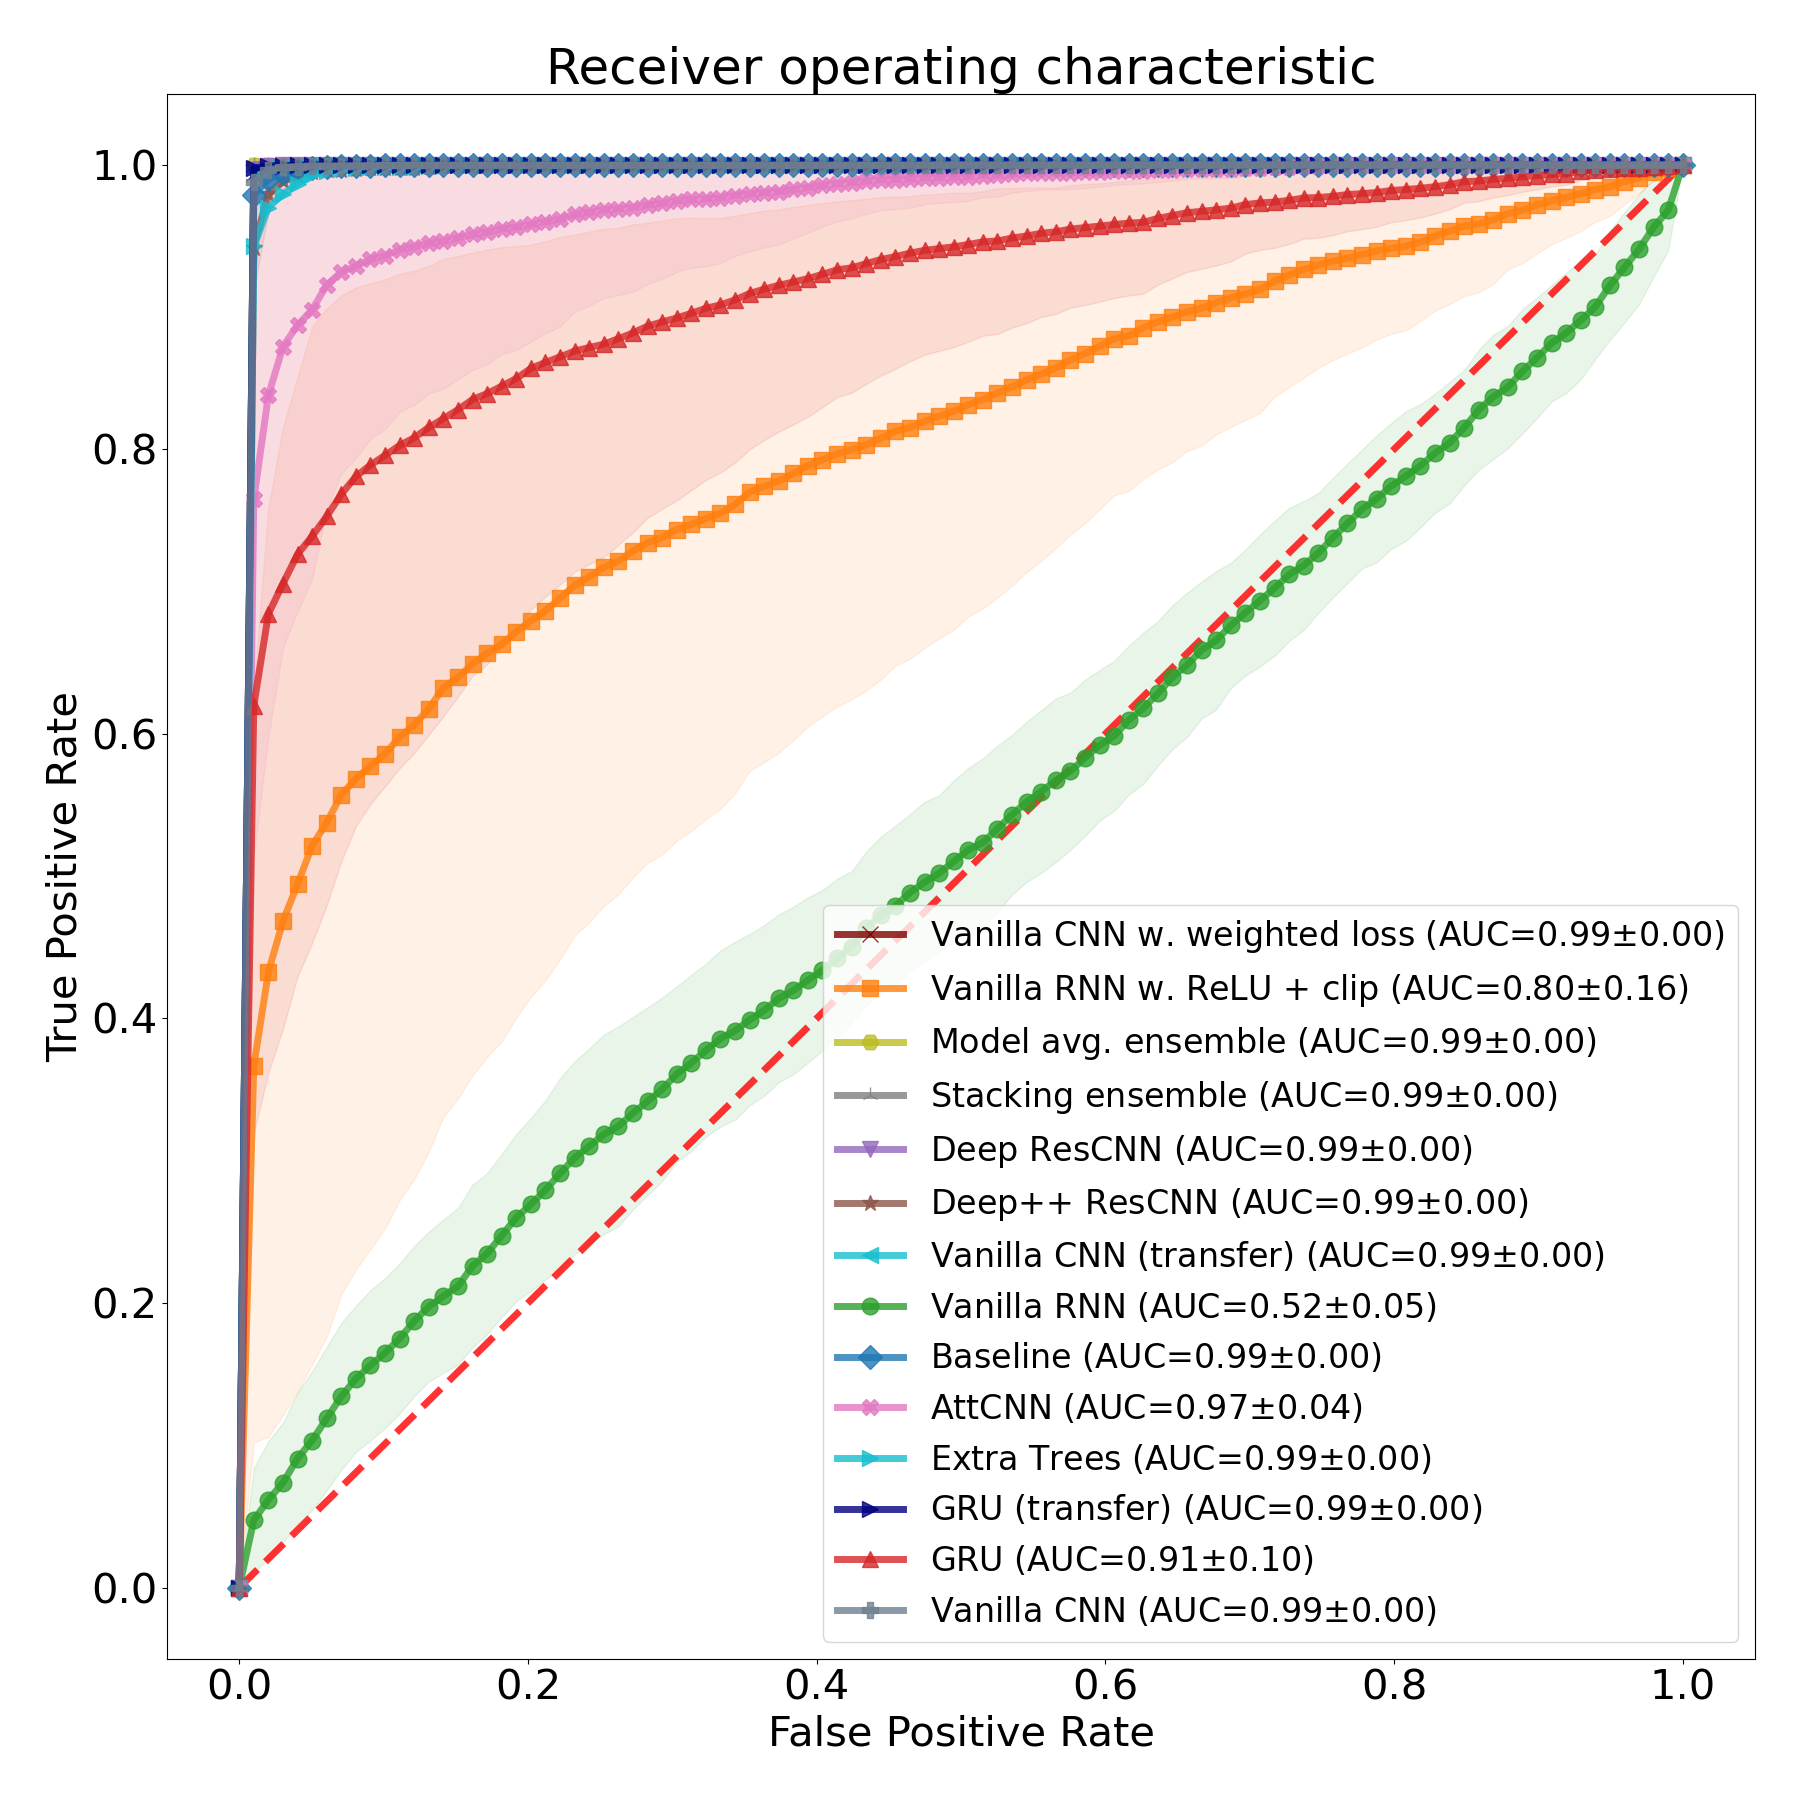
\includegraphics[width=0.3\textwidth]{figures/roc_ptbdb.png}
    \caption{Receiver operating characteristic curve for our models on the PTB DB test dataset. The shaded areas depict \boldmath$\pm 1$ standard deviation from the mean.}
    \label{fig:roc_ptbdb}
\end{figure}

\subsubsection{Test scores}
\autoref{tab:results_ptbdb} and \autoref{tab:results_mitbih} show the performance metrics on the test sets. Generally, we observe good performance close to the baseline for most models. Notably our \textsc{VanillaCNN} shows good performance, outperforming the baseline on both datasets. However, adding model complexity does not yield better results as evident by the performance of \textsc{Deep++ ResCNN} and \textsc{AttCNN}.

In line with the observed stagnating loss, \textsc{VanillaRNN} with Tanh activation and no gradient clipping fails to produce useful outputs for both datasets. As seen in the confusion matrix in \autoref{fig:confusion_matrices_mitbih} as well as the ROC curve in \autoref{fig:roc_ptbdb}, it is clear that it does not perform better than random chance. The RNN-based models, \textsc{VanillaRNN+ReLU+Clip} and \textsc{GRU}, perform much better, especially on the MIT-BIH dataset. On the smaller PTB DB dataset they lack performance. This can likely be explained by the fact that they require more training data due to a large amount of parameters. This may also help explain why \textsc{GRU} benefits greatly from transfer learning, outperforming all other non-ensemble models on PTB DB. The smaller \textsc{VanillaCNN} does not benefit as much from transfer learning, showing only a small improvement.

The tree-based models, \textsc{Extra Trees}, produce predictions that are useful, yet not competitive with the baseline. They, however, train much faster than the deep learning models leading to a trade-off between performance and training time.

As seen in \autoref{fig:confusion_matrices_mitbih}, a weighted loss may balance class frequency effects as shown by the improved performance for \textsc{VanillaCNN} in predicting minority classes after being trained with the weighted loss. Overall accuracy and F1 score does decrease as another trade-off. We note that this behavior may be desired in some settings where, e.g., false negatives are more problematic for specific classes such as in medical domains.

Finally, as expected, the ensemble methods building upon all models and their variations perform very well. Both of their accuracies are within around a standard deviation of the best performing model on both datasets, outperforming all other models at times. Still, \autoref{fig:confusion_matrices_mitbih} shows that the ensemble methods inherit the minority class inaccuracies of the models that they build upon.


\section{Conclusion}
\label{sec:conclusion}

In this work, we investigated the performance of several deep-learning based models across the tasks of ECG interpretation and heart arrhythmia classification. Having benchmarked all of our models, we showed that a simple CNN model is able to achieve good performance on both tasks and added model complexity may not yield better results. Further, introducing class weights on the loss can lead to better results for minority classes trading off some overall performance. Finally, we showed that model performance can be improved using transfer learning or ensemble methods across diverse models but these may inherit problems from the sub-learners such as decreased performance across rare events or classes. 


\begin{table*}[]
\centering
\addtolength{\leftskip} {-2cm}
\addtolength{\rightskip}{-2cm}
\sisetup{
table-alignment-mode = format
}
\begin{tabular}{@{}
  l
  S[table-format=3.0(3)]
  S[table-format=1.4(1)]
  S[table-format=1.4(1)]
  S[table-format=1.4(1)]
  S[table-format=1.4(1)]
  @{}}
\toprule
Model & {Training time (s)} & {Accuracy} & {F1} & {AUROC} & {AUPRC} \\
\midrule
\textsc{Stacking ensemble} & 583 \pm 10 & \bfseries 0.9969 \pm 0.0000 & \bfseries 0.9961 \pm 0.0000 & \bfseries 0.9989 \pm 0.0000 & \bfseries 0.9995 \pm 0.0000 \\
\textsc{GRU} (transfer) & 321 \pm 30 & 0.9954 \pm 0.0011 & 0.9943 \pm 0.0014 & 0.9988 \pm 0.0002 & 0.9993 \pm 0.0002 \\
\textsc{Deep ResCNN} & 52 \pm 11 & 0.9951 \pm 0.0011 & 0.9938 \pm 0.0013 & 0.9971 \pm 0.0002 & 0.9973 \pm 0.0003 \\
\textsc{Model avg. ensemble} & & 0.9945 \pm 0.0000 & 0.9931 \pm 0.0000 & 0.9981 \pm 0.0000 & 0.9988 \pm 0.0000 \\
\textsc{VanillaCNN} (transfer) & 35 \pm 9 & 0.9945 \pm 0.0011 & 0.9931 \pm 0.0014 & 0.9975 \pm 0.0006 & 0.9982 \pm 0.0005 \\
\textsc{VanillaCNN} w. weighted loss & 41 \pm 9 & 0.9937 \pm 0.0014 & 0.9921 \pm 0.0017 & 0.9966 \pm 0.0004 & 0.9973 \pm 0.0004 \\
\textsc{VanillaCNN} & 39 \pm 7 & 0.9926 \pm 0.0016 & 0.9907 \pm 0.0020 & 0.9967 \pm 0.0007 & 0.9975 \pm 0.0006 \\
\textsc{Baseline} & 49 \pm 9 & 0.9893 \pm 0.0042 & 0.9866 \pm 0.0053 & 0.9981 \pm 0.0009 & 0.9991 \pm 0.0005 \\
\textsc{Deep++ ResCNN} & 72 \pm 7 & 0.9842 \pm 0.0048 & 0.9802 \pm 0.0060 & 0.9966 \pm 0.0015 & 0.9984 \pm 0.0009 \\
\textsc{Extra Trees} & \bfseries 12 \pm 0 & 0.9799 \pm 0.0005 & 0.9747 \pm 0.0006 & 0.9963 \pm 0.0001 & 0.9982 \pm 0.0001 \\
\textsc{AttCNN} & 95 \pm 30 & 0.9504 \pm 0.0604 & 0.9310 \pm 0.0893 & 0.9734 \pm 0.0429 & 0.9881 \pm 0.0188 \\
\textsc{GRU} & 328 \pm 111 & 0.8850 \pm 0.1055 & 0.8440 \pm 0.1468 & 0.9135 \pm 0.0971 & 0.9636 \pm 0.0409 \\
\textsc{VanillaRNN+ReLU+Clip} & 356 \pm 279 & 0.8201 \pm 0.1200 & 0.6350 \pm 0.2642 & 0.8032 \pm 0.1582 & 0.9096 \pm 0.0742 \\
\textsc{VanillaRNN} & 134 \pm 18 & 0.7221 \pm 0.0000 & 0.4193 \pm 0.0000 & 0.5166 \pm 0.0476 & 0.7559 \pm 0.0374 \\
\bottomrule
\end{tabular}
\caption{Model performances on the PTB DB test dataset.\protect\footnotemark{\label{footnote:ensemble}}}
\label{tab:results_ptbdb}
\end{table*}

\footnotetext{Note that the ensemble models require all other models to be trained beforehand as they are trained on their prediction outputs. The training times are therefore not directly comparative to other models.}


\begin{table*}[]
\centering
\sisetup{
table-alignment-mode = format
}
\begin{tabular}{@{}
  l
  S[table-format=4.0(1)]
  S[table-format=1.4(1)]
  S[table-format=1.4(1)]
  @{}}
\toprule
Model & {Training time (s)} & {Accuracy} & {F1} \\
\midrule
\textsc{Model avg. ensemble} & & \bfseries 0.9875 \pm 0.0000 & 0.9247 \pm 0.0000 \\
\textsc{VanillaCNN} & 181 \pm 31 & 0.9874 \pm 0.0008 & 0.9248 \pm 0.0058 \\
\textsc{GRU} & 1775 \pm 239 & 0.9872 \pm 0.0007 & \bfseries 0.9251 \pm 0.0049 \\
\textsc{Stacking ensemble} & 3818 \pm 62 & 0.9870 \pm 0.0000 & 0.9211 \pm 0.0000 \\
\textsc{Deep ResCNN} & 321 \pm 45 & 0.9864 \pm 0.0006 & 0.9199 \pm 0.0026 \\
\textsc{Baseline} & 290 \pm 33 & 0.9850 \pm 0.0009 & 0.9143 \pm 0.0040 \\
\textsc{Deep++ ResCNN} & 442 \pm 65 & 0.9849 \pm 0.0011 & 0.9147 \pm 0.0066 \\
\textsc{AttCNN} & 577 \pm 138 & 0.9836 \pm 0.0012 & 0.9076 \pm 0.0084 \\
\textsc{Extra Trees} & \bfseries 67 \pm 7 & 0.9764 \pm 0.0002 & 0.8792 \pm 0.0022 \\
\textsc{VanillaCNN} w. weighted loss & 260 \pm 39 & 0.9681 \pm 0.0027 & 0.8554 \pm 0.0074 \\
\textsc{VanillaRNN+ReLU+Clip} & 2994 \pm 1911 & 0.9543 \pm 0.0224 & 0.7443 \pm 0.1483 \\
\textsc{VanillaRNN} & 886 \pm 84 & 0.8306 \pm 0.0060 & 0.1972 \pm 0.0322 \\
\bottomrule
\end{tabular}
\caption{Model performances on the MITBIH test dataset.\protect\footnotemark}
\label{tab:results_mitbih}
\end{table*}


\footnotetext{See footnote \ref{footnote:ensemble}.}





\bibliographystyle{ACM-Reference-Format}

\bibliography{bibliography}

\clearpage
\newpage
\appendix

\section{Misclassified SHAP images}
\label{sec:appendix_misclassified}
\autoref{fig:appendix_shap} shows misclassifications for our CNN baseline and VGG16 transfer learning model.

\begin{figure*}[b]
\centering
\begin{subfigure}{0.5\linewidth}
  \centering
    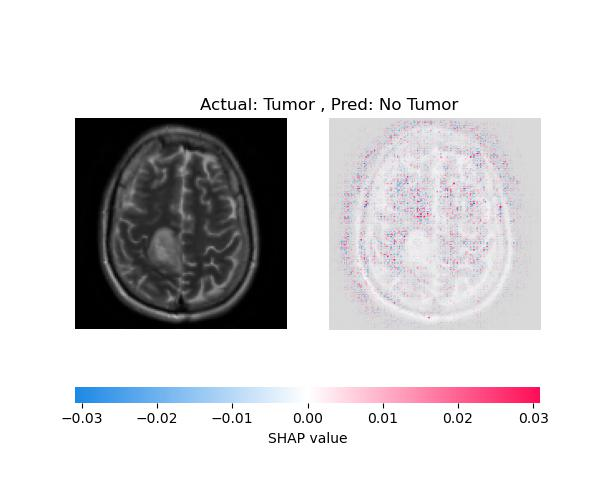
\includegraphics[width=1\linewidth]{figures/baseline_cnn_incorrect_shap.jpeg}
    \caption{}
    \label{fig:baseline_cnn_incorrect_shap}
\end{subfigure}%
\begin{subfigure}{0.5\linewidth}
  \centering
    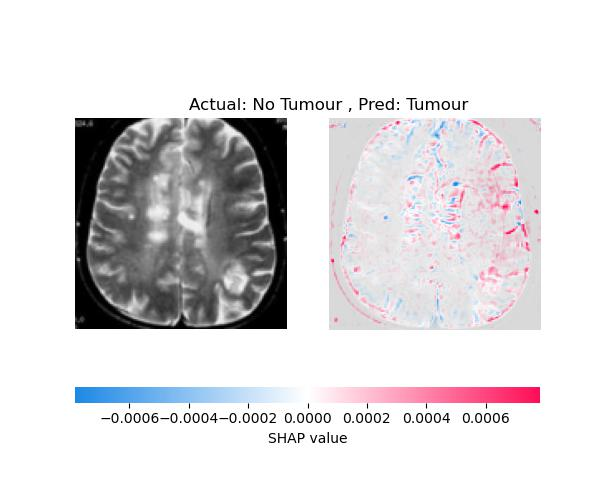
\includegraphics[width=1\linewidth]{figures/transfer_learning_incorrect_shap.jpeg}
    \caption{}
    \label{fig:transfer_learning_incorrect_shap}
\end{subfigure}
\caption{SHAP images. (a) \textsc{Baseline CNN} (Actual: Tumor, Pred: No Tumor). (b) \textsc{VGG16 TL} (Actual: No Tumor, Pred: Tumor).}
\label{fig:appendix_shap}
\end{figure*}


\end{document}
